\documentclass[onecolumn, draftclsnofoot,10pt, compsoc]{IEEEtran}
\usepackage{graphicx}
\usepackage{url}
\usepackage{setspace}
\usepackage{csquotes}
\usepackage{float}
\usepackage{soul}
\usepackage{color}
\usepackage{pstricks-add}

\usepackage{listings}

% COLOR DEFINITIONS FOR CODE LISTINGS
\definecolor{codegreen}{rgb}{0,0.6,0}
\definecolor{codegray}{rgb}{0.5,0.5,0.5}
\definecolor{codepurple}{rgb}{0.58,0,0.82}
\definecolor{backcolour}{rgb}{0.95,0.95,0.92}

\lstdefinestyle{mystyle}{
    backgroundcolor=\color{backcolour},
    commentstyle=\color{codegreen},
    keywordstyle=\color{magenta},
    numberstyle=\tiny\color{codegray},
    stringstyle=\color{codepurple},
    basicstyle=\footnotesize,
    breakatwhitespace=false,
    breaklines=true,
    captionpos=b,
    keepspaces=true,
    numbers=left,
    numbersep=5pt,
    showspaces=false,
    showstringspaces=false,
    showtabs=false,
    tabsize=2
}

\lstset{
	escapeinside={(*@}{@*)},
	style=mystyle
}

\usepackage{geometry}
\geometry{textheight=9.5in, textwidth=7in}

% 1. Fill in these details
\def \CapstoneTeamName{	Short Circuit Comedy Club	}
\def \CapstoneTeamNumber{		CS13}
\def \GroupMemberOne{			Kevin Talik}
\def \GroupMemberTwo{			Arthur Shing}
\def \GroupMemberThree{			Anish Asrani}
\def \CapstoneProjectName{		How to Build an Effective Robot Comedian}
\def \CapstoneSponsorCompany{	Oregon State University}
\def \CapstoneSponsorPerson{		Dr. Heather Knight}

% 2. Uncomment the appropriate line below so that the document type works
\def \DocType{		%Problem Statement
				%Requirements Document
				%Technology Review
				%Design Document
				Final Document
				}

\newcommand{\NameSigPair}[1]{\par
\makebox[2.75in][r]{#1} \hfil 	\makebox[3.25in]{\makebox[2.25in]{\hrulefill} \hfill		\makebox[.75in]{\hrulefill}}
\par\vspace{-12pt} \textit{\tiny\noindent
\makebox[2.75in]{} \hfil		\makebox[3.25in]{\makebox[2.25in][r]{Signature} \hfill	\makebox[.75in][r]{Date}}}}
% 3. If the document is not to be signed, uncomment the RENEWcommand below
%\renewcommand{\NameSigPair}[1]{#1}

%%%%%%%%%%%%%%%%%%%%%%%%%%%%%%%%%%%%%%%
\begin{document}
\begin{titlepage}
    \pagenumbering{gobble}
    \begin{singlespace}
 %   	\includegraphics[height=4cm]{coe_v_spot1}
        \hfill
        % 4. If you have a logo, use this includegraphics command to put it on the coversheet.
        %\includegraphics[height=4cm]{CompanyLogo}
        \par\vspace{.2in}
        \centering
        \scshape{
            \huge CS Capstone \DocType \par
            {\large\today}\par
            \vspace{.5in}
            \textbf{\Huge\CapstoneProjectName}\par
            \vfill
            {\large Prepared for}\par
            \Huge \CapstoneSponsorCompany\par
            \vspace{5pt}
            {\large Prepared by }\par
            Group\CapstoneTeamNumber\par
            % 5. comment out the line below this one if you do not wish to name your team
            \CapstoneTeamName\par
            \vspace{5pt}
            \vspace{20pt}
        }
        \begin{abstract}
  	     % 6. Fill in your abstract
			The purpose of this document is to outline the research papers that this team will create to conclude during Spring Term 2018.
			The three members of the \textit{Short Circut Comedy Club} have spent their time during winter term perfomring research under Dr. Heather Knight at Oregon State University.
			The focus of this project is to study the effect a robot comedian can have on a crowd of humans.
			Kevin Talik's research has been spent understanding what a Comedian can do to "Adapt" to a performance.
			Arthur Shing has been studying the voice of the robot, and the difference between "Robot and Human" character.
			One final aspect of Stand-Up Comedy that we studied is "Crowd Work". Anish Asrani has spent most of his time developing spontaneous Crowd-Interactions during the set.
        \end{abstract}
    \end{singlespace}
\end{titlepage}
\newpage
\pagenumbering{arabic}
\tableofcontents
% 7. uncomment this (if applicable). Consider adding a page break.
%\listoffigures
%\listoftables
\clearpage

\section{Introduction to Project}
Who requested it?
Why was it requested?
What is its importance?
Who was/were your client(s)?
Who are the members of your team?
What were their roles?
What was the role of the client(s)? (I.e., did they supervise only, or did they participate in doing development)

\section{Introduction - Requirements}
The field of human-robot interaction can learn a lot from stand-up comedy. A stand-up performance has a basis of scripted content, from which the comedian delivers jokes to engage the audience. Good Comedians can read the audience and sometimes adapt their delivery based on the mood of the room \cite{talkingFunny}. In social robotics, when a robot shares a space with a human, an interaction can influence the people's opinions of the robot. Additionally, evident character traits presented (through dialogue and non-verbal motion) by the machine can anthropomorphize itself, making it easier and more enjoyable to connect with for the human \cite{KnightEightLessons:2011}. The purpose of this work is to explicitly evaluate what aspects of a robot comedian's performance are most salient to human audience.


\section{Previous Research}

Research on the improvement of HRI is indispensable for our project. In Heather Knight's \textit{Eight Lessons}, gestures, liveliness, and joke timing are all aspects that can be incorporated into the robot {\cite{KnightEightLessons:2011}}.
Relatable and appropriate gestures significantly helps improve communication between the robot and the audience. If the actions are predictable, humans can relate to the robot.
When watching someone perform an action, the human brain maps the actions onto itself and simulates the action in the best way possible. This is a physiological experience that should be replicated by the robot in order to enhance relatability. Simplicity is important as well. {\cite{KnightEightLessons:2011}}

In addition, Knight observed that having the robot portrayed as a living character rather than just an object that is kept up on stage improved the overall experience for the observers. Having believable interactions can enhance the feeling of a living character.
The goal of the audience tracking using sensors is to maximize enjoyment. The enjoyment levels were be read by the robot and used to modify upcoming jokes {\cite{KnightEightLessons:2011}}. Pausing and letting the audience laugh is vital as well. Starting the next joke too early can break the rhythm and leave the audience baffled. Looking around and body poses should be used to fill the pause {\cite{KnightEightLessons:2011}}.

In a previous study of robot comedy \cite{RobotComedyLab:2015}, Katevas found that when a robot engaged the audience through eye contact, the audience was more receptive to the performance. Eye contact from the robot is important, as it is a non-verbal cue for direct interaction. The audience members can identify that the machine is making an attempt to engage with specific members of the audience. We will investigate this further by having the robot perform various non-verbal and verbal interactions using sensors. The idea is to have the audience be a part of the performance even if they are not the ones performing. This can be accomplished if the robot is socially intelligent.

Other studies by Katevas et al. \cite{KatevasRobot:2014} that involved evaluating the social dynamics of a live performance by a robot have used SHORE\textsuperscript{TM} vision framework software to analyze and detect faces in the audience. SHORE\textsuperscript{TM} allows for facial expression recognition, estimated age, gender, and eye or mouth openings \cite{SHORE}, giving the study a heterogeneous audience model. These allowed for the robot to interact directly with specific audience members. However, usage of SHORE\textsuperscript{TM} involves expenses and funds that are unavailable to us, so we will encounter behavioral limitations dealing with a homogeneous audience model.

A study by Guy Hoffman {\cite{hoffman2010anticipation}} noted the importance of anticipation in human-robot interaction (HRI). The timing and meshing of anticipatory action and perception are a useful framework for HRI. The greatest challenge when designing a robot that will perform on stage is to enable the robot to be both - expressive and responsive. Robot models in the past have ended up on either extreme; they are either real-time and do not allow for continuous expression, or they are very animated but do not allow well times reactive behavior.


Researchers have also proposed multiple design patterns to promote sociability in Human-Robot Interaction (HRI). Some of these include having an initial introduction, some sort of didactic communication, including personal interests or history, and recovering from mistakes \cite{Kahn:2008}. These patterns in design are proposed to allow for more effective and meaningful social interactions. While there is yet to be much data or research on the validity of these claims, they may still prove to be useful in guiding the designs of our project.


% The effectiveness of our robot comedian will be evaluated by human enjoyment levels. Specifics regarding measurements and analysis will be later discussed with the client. Some possible methods include handing out surveys for the audience to fill out, which may include questions regarding the subjective reception of the robot comedian. Additionally, behavioral statistics may be used to evaluate the effectiveness of the comedy.

Robots utilizing non-verbal communication and statically written audience engagement have been attempted in robot comedy. In particular, Knight has observed the importance of character and spontaneous interactions in creating effective comedy \cite{KnightEightLessons:2011}. However, there is little research on the actual effectiveness of character and spontaneous interactions \cite{KatevasRobot:2014}. This project will aim to examine the effectiveness of character and spontaneous interactions in robot comedy.

\section{Hypothesis}

Our research will be guided by the following questions:
\begin{enumerate}[\IEEEsetlabelwidth{6)}]
\item How can the robot make the audience feel like a part of the performance?
\item How can the robot convey and a coherent and well-developed character?
\item How can the robot adapt and influence to the audience?
\end{enumerate}

We hypothesize that comedy scripts with greater degrees of (1) crowdwork, (2) character, and (3) adaptiveness, will create more effective comedy, and have a more positive response from the audience.

\subsection{Crowdwork}
% TODO: Explain why crowdwork might have effects (reference 8 lessons?) and what crowdwork might look like in a script

Keeping the audience engaged is vital in creating an entertaining performance. Katevas et al. had some success leading to a better audience response when using gestures and acknowledging the audience's presence. A successful performance manages the dynamics of various aspects of interaction to the benefit of both the performer and the audience \cite{RobotComedyLab:2015}. Interaction with the audience will make the comedian robot feel more authentic, like an entity, and less like an object. Knight's research found that the robot's connection with the audience is stronger if the robot is able to convey social intelligence. This helps the robot display that it is not just an inanimate object \cite {KnightEightLessons:2011}.

\subsection{Character}
% TODO: Find a better place to put this? Maybe it fits here
Expressing character will be understood from the robot under the "theory of the mind" \cite{leslie}. Understanding the agents meta-representation of a behavior is helpful for the audience in relating to the robot's intent, desires and knowledge. A robot attempts this to understand and relate its desires and intent better to the audience \cite{theoryOfMindRobots}.


% TODO: Explain why character might have effects (reference 8 lessons?) and what character might look like in a script
The appearance of character in a robot may create more effective comedy.
Research has shown that expressive behaviors in a robot may cause interacting humans to favor the robot \cite{DesignExBeh:2017}.
One could argue that expressive behaviors are behavioral actions formed by an inner character. While robots currently are not capable of having intrinsic character qualities, we postulate that a robot which behaves as if it has character could be more effective at engaging an audience. The task of conveying a sense of character may also benefit from social behaviors developed in researching the effectiveness of crowdwork, as social interactions may increase the sense of agency \cite{KnightEightLessons:2011} and thus aid the audience in grouping behaviors as acts of character.




\subsection{Adaptiveness}

% TODO: Explain why adaptiveness might have effects (reference 8 lessons?) and what adaptivity might look like in a script



When the robot tells a joke, it needs to make adaptive transitions that correlates with the response. For example, if a joke does well and is received with laughter, the robot needs to time the next joke so that it is delivering it when the audience is ready, and can hear. However, if a joke is not well received by the audience, the time a robot needs to wait for the next joke will be different than if there is laughter. This is important for the effectiveness of a performance, as the connotation of the next joke is determined by the result of the previous joke; an audience that is told a bad joke will be hesitant to enjoy a joke if the previous jokes were bad. A robot comedian needs to be able to stay in a joke if the audience likes it, or address/recover the bad joke before starting a new sequence. Timing, or anticipation for a new joke, when coordinated correctly, positively influences the fluidity of the task (the performance) \cite{hoffman2010anticipation}.


\section{Research Approach}
This project will be carried out in three phases; A learning and exploration phase in Fall term, a prototyping and testing phase in the Winter, and our evaluation phase Spring term.

\subsection{Learning/Exploration Phase}
This phase of our development will focus on understanding Social Robotics and the technology of the robot. The three of us will become familiar with stand-up comedy and the dynamics of an audience-comedian interaction. The NAO robot behaviors are programmed in the software Choregraphe, which has an API for python. We will test primitive scripts of decision making and non-verbal behavior. This is to learn how the coding environment works and to familiarize ourselves with hardware limitations. Additionally, we will learn to work with the sensors on the robot, and how they function (microphone, camera, etc). To become familiar with the format of a stand-up performance, we intend to study jokes and comedy devices.

\subsection{Prototyping/Testing Phase}
In the prototyping and testing phase, we will develop early sets for the robot. These implementations need to reflect and support our research questions. Crowd-work will involve audience sensing, as well as jokes that incorporate a measurement of response from the audience. Character implementation will involve testing the differences in effectiveness of robot vs human joke delivery, and the effectiveness of robo-centric jokes. As a stretch goal, we also hope to prototype and test the effectiveness of adapting a set to the audience, using intelligent calibration of the sensors.

These prototypes will be in the form of 3-6 minute set scripts with several variants in Choregraphe. The variants will help us evaluate the research questions and can be be tested in front of a small sample of humans, or in the form of a video recording. For example, the robot may perform in front of a handful of friends, or recordings may be to show online live viewers. Non-mechanical feedback from our testing will influence the direction of our prototyping, meaning that the implementation of our research questions will adapt according to the audience response. By the time this phase is completed, we will have working sets of robot stand-up.

\subsection{Evaluation Phase}
While doing the research, we will perform 6 shows with audiences ranging from 10-30 people. Tests in this phase will be at a greater scale and with a more realistic environment. Each stand-up performance, or set, will contain bits, or sections of content that will be categorized as crowd work, characterization dialogue, and jokes. We will be testing on a live human audience to learn the effectiveness of each bit in a set. Based of the effectiveness of each set, we will modify the set and behavior of the robot. By the end of this phase, we hope to have a working, effective robot comedian.

\section{Methods}

% Experiment Design,
% Algorithms for Adaptive Behavior,
% Behavioral Statistics, whatever the hell that is
\subsection{Tests}

Our research questions will be how we evaluate the effectiveness of a robot comedian.
We will create performances with varying degrees of (1) crowdwork, (2) character, and (3) adaptiveness. We will vary the presence of each of the factors of the performance to determine which factors are most influential to the comedian.
To test crowdwork, we may create one script may include no references to the audience (low degree of crowdwork), while another may include many instances of interactions with the audience (high degree of crowdwork).
% Example of interaction in script
% For instance, an interaction with the audience may include lines such as, "You guys look great today!"
To test the effectiveness of adding character, we may create a script with random jokes (low degree of character), and one with a coherent character throughout the set (high degree of character).


Likewise, testing the effectiveness of adaptivity will include scripts with no adaptivity and scripts that adjust to audience response.These scripts will be run on the NAO robot, and performed in front of a small audience in the testing phase, and later a larger live audience in the evaluation phase.

The audio sensors on the NAO bot will be used to evaluate audience reception to a joke, which the robot can then adapt to. The microphone on the NAO does not perform well when receiving input from a large audience, as it is designed to handle smaller scale interactions. NAO interprets speech with the ALSpeechRecognitionProxy and ALTextToSpeechProxy \cite{audiodocs}.


\subsection{Metrics}

To evaluate the effectiveness of our robot comedian, we will measure the response of the performance with the audio captured during the set, and surveys for the audience afterwards. Measuring the audio will help us understand a broad audience response, as well as data for adaptive functionality. Surveys will give a more in depth information on factors of the show that are not covered by audio sensing, such as opinions of the perceived character and quality of the jokes. For example, to see if the robot’s character was conveyed coherently, the audience will fill out a questionnaire prompting them to describe its character, as well as some humanizing questions, e.g. "Would you invite this robot to dinner?" These responses will be used to study if the robot matched the expected persona and gauge how comfortable the people are with the robot.


As each set will derive content from the three research questions, we need to measure the effectiveness of each portion compared across the 6 performances. The survey that the audience members take after the show will gauge the response to sections. Additionally, there will need to be questions to establish a pretense of how an audience member felt before the show, and how the performance has influenced their opinions of robot comedy. We want to see if someone who has seen a robot comedian would recommend the show to others.

The microphone on the NAO robot is designed for small environment settings. It will be difficult to distinguish speech from separate sources in a noisy environment \cite{alsounddetection}. Audio levels will be important data to collect from a crowd, where a louder crowd response could correlate to a level of enjoyment. However, a problem could be that a crowd could be booing very loud, and if we do not distinguish between different sounds that the audience can make, we could accidentally associate a negative response with a good response. The background noise could be very different depending on the room size. The density of people in a room making noise may return different audio level \cite{alsoundlocalization}. It will be important to test the effectiveness of a microphone to receive input.

\section{Conclusion}
A stage presence for a comedian is important because it connects the audience to the content, making it more effective than soulless delivery. A robot has a disadvantage in this; being soulless is the essence of being a robot. For a robot to establish a stage presence, the machine needs to make efforts to connect with the crowd, present a cohesive character, and dynamically adapt to a response. We think that a round character personifies a relatable agent for an audience. If a robot can give insight to it's desires, behavior, and preferences during a performance, the robot will humanize itself, connecting itself to the crowd.

\clearpage

  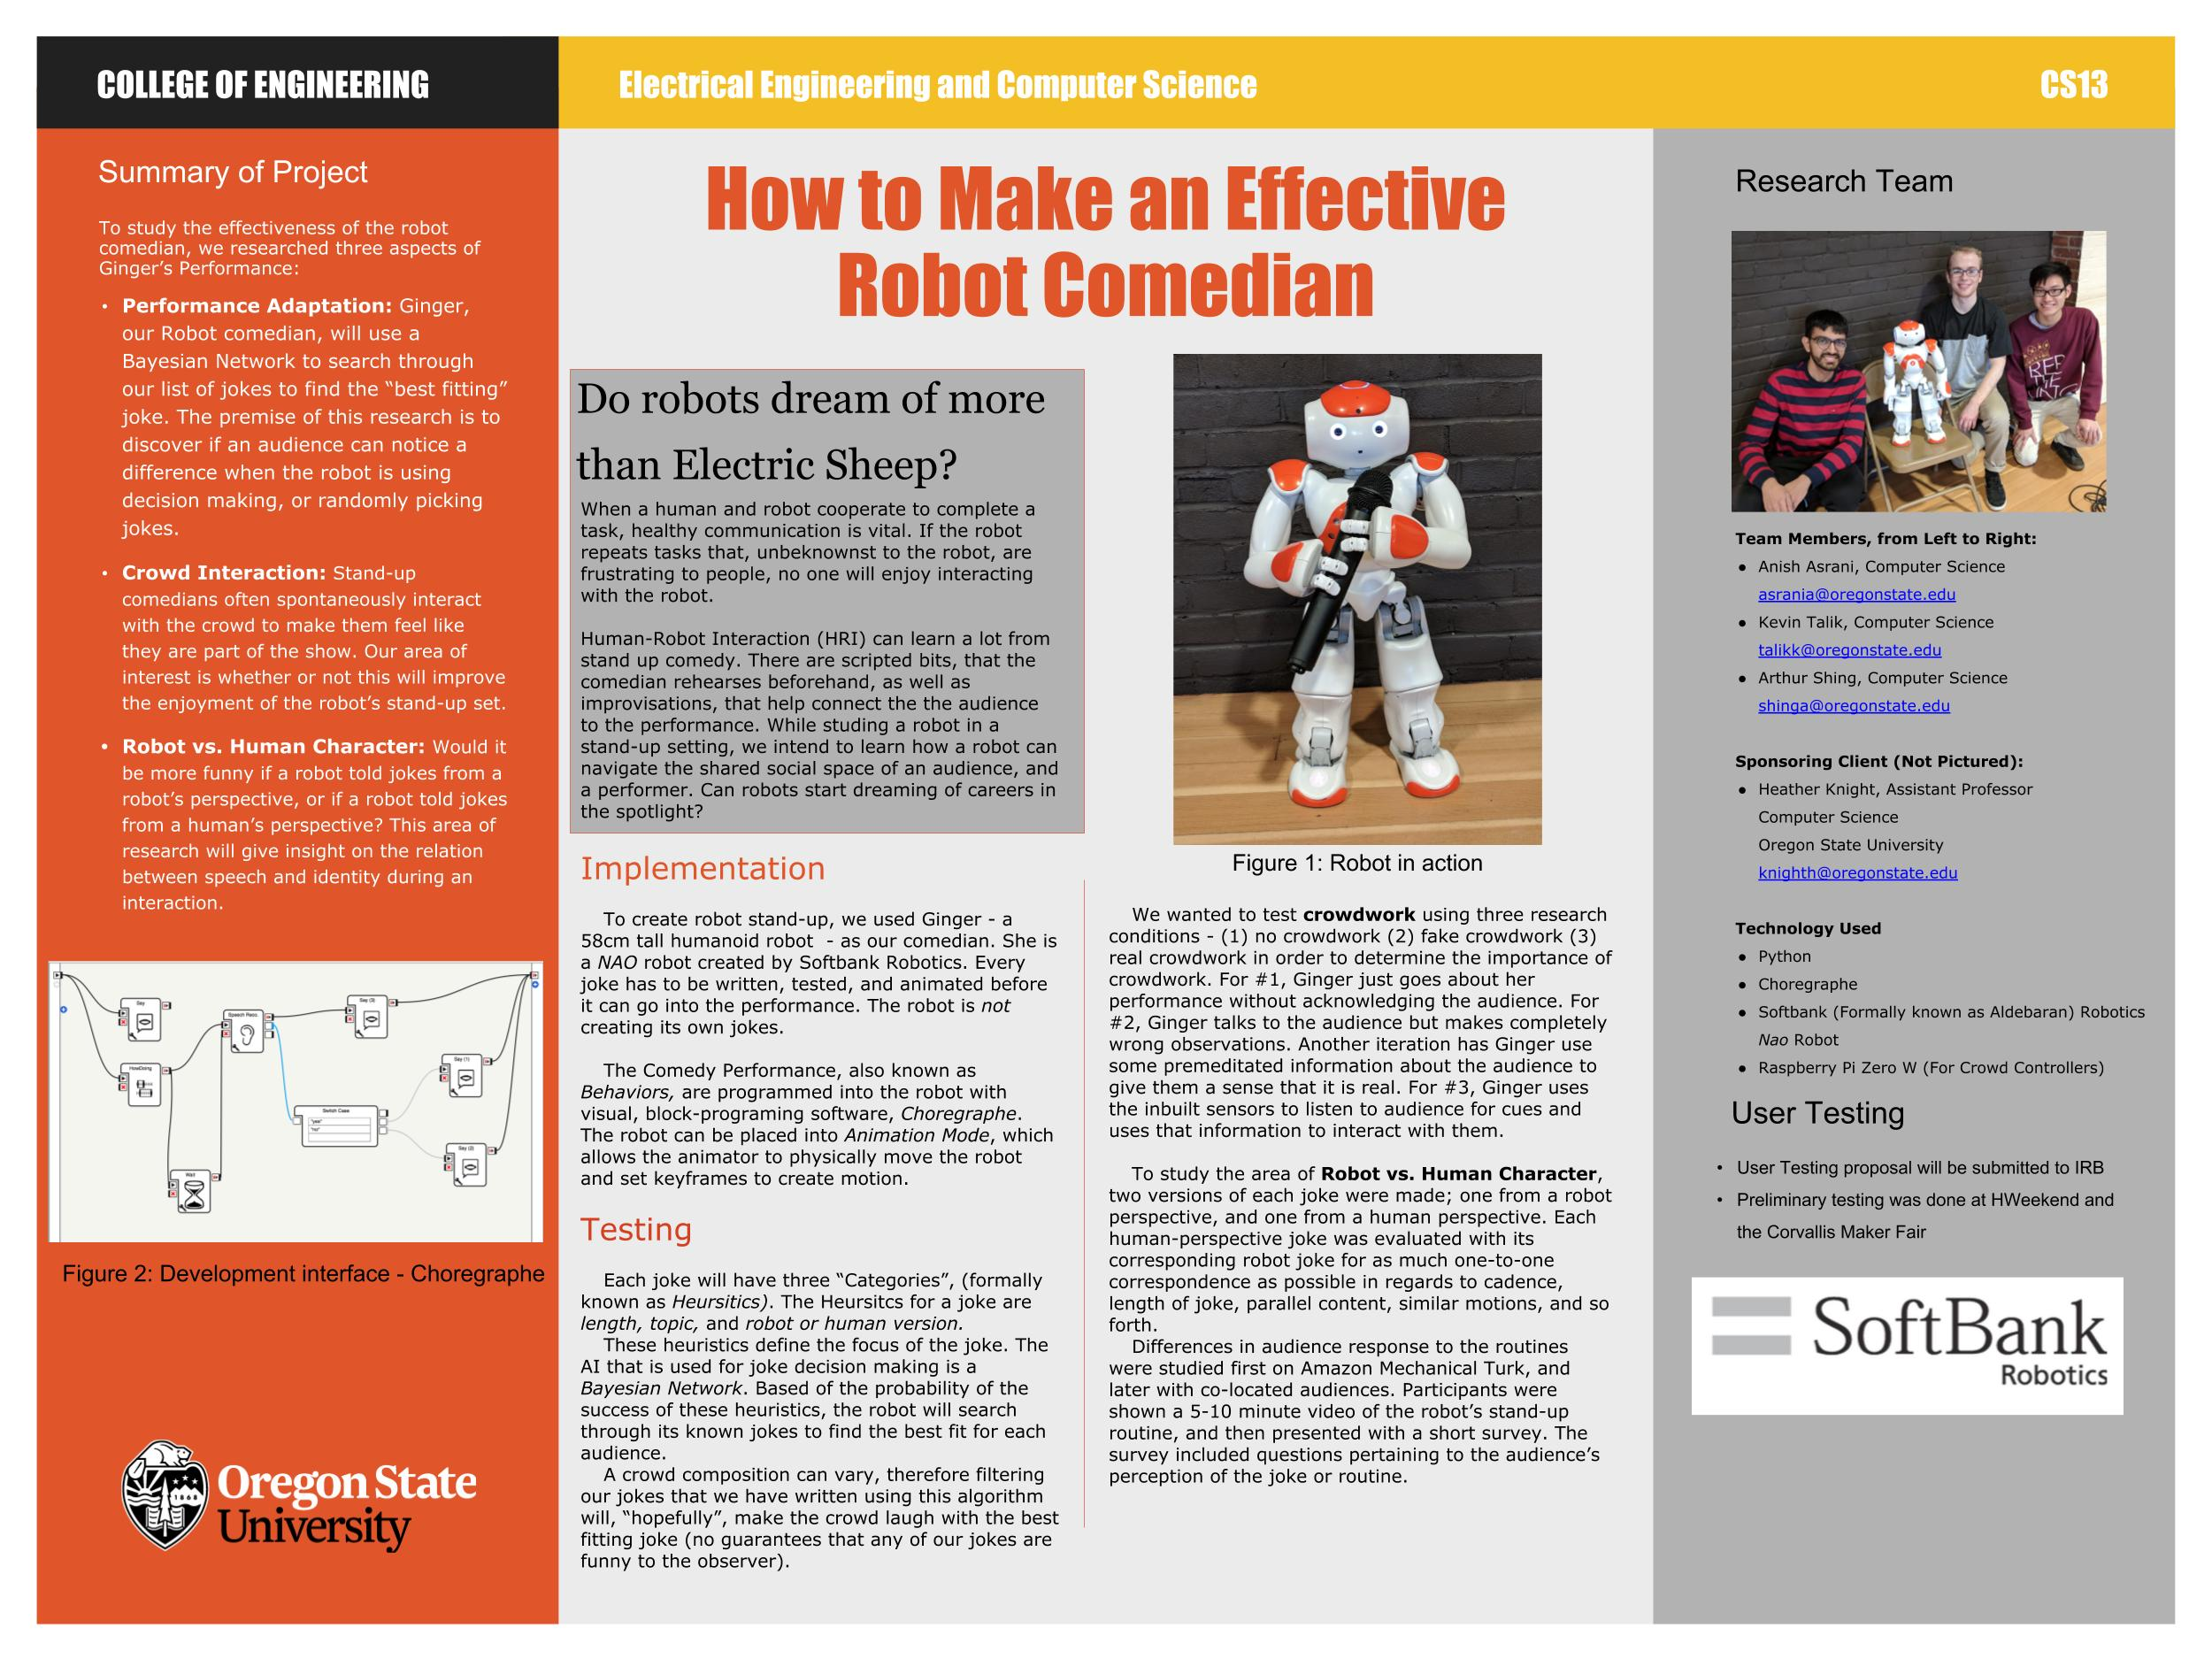
\includegraphics[width=\textwidth]{poster.jpg}


\end{document}
